% 2009-10-06  Michele Tavella <michele.tavella@epfl.ch>
\documentclass[a4paper,10pt]{article}
%\usepackage{hyperref}
\usepackage{color}
\usepackage{graphicx}
\usepackage{subfigure}
\usepackage{verbatim}
\usepackage[numbered,autolinebreaks,useliterate]{mcode}

\newcommand{\temp}[1]{\textcolor{blue}{\textbf{#1}}}
\newcommand{\note}[1]{\textcolor{red}{#1}}
\newcommand{\blame}[1]{\textbf{#1}}
\graphicspath{{images/}}

\hyphenpenalty=5000
\tolerance=1000

\title{TOBI iC\\
\large{Definition, implementation and scenarios}}
\author{Michele~Tavella\\
\footnotesize{\texttt{michele.tavella@epfl.ch}}}

\begin{document}
\date{\today}
\maketitle
\tableofcontents 
\pagebreak

\section{Introduction}
The TOBI iC is designed by TOBI's WP5 and WP8 members, while its implementation
is mantained by EPFL.
iC defines the way classifiers in the hBCI transmit their outputs to other
modules.
The core component of iC is the ``iC message``. An iC message is the atomic
unit used by the hBCI to transmit classifier outputs. 
An iC message can encode the outputs of multiple classifiers, regressors etc.
As today, iC is available as a C++ library (Section~\ref{sec:libtobiic}) and as
a MEX interface (Section~\ref{sec:mextobiic}).
Under this perspective it is safe to assume that only data with a high
information content but with a reduced transmission rate have to be handled by
this interface. 

\subsection{Disclaimer}
\label{sec:disclaimer}
The goal of this document is to make users familiar with hBCI designs including
iC. The document is written in an easy format that should be familiar to most of
the BCI community, thus not only addressing the hBCI-ninjas within the TOBI
consortium or the code-monkeys in your lab.
This document is shipped with the iC library libtobiic and it has to be
considered an evolving text that will be continuously updated.
Although it contains some references and examples based on libtobiic and
mextobiic, this document does not replace the Doxygen or Matlab documentation
shipped with libtobiic and mextobiic respectively.

\subsection{Acknowledgment}
\label{sec:acknowledgment}
This work is supported by the European ICT Programme Project FP7-224631,
TOBI: Tools for Brain-Computer Interaction. This document only reflects the
authors' views and funding agencies are not liable for any use that may
be made of the information contained herein.

\section{iC and the hBCI}
\label{sec:hbci}
Before moving to the design details, it is important to highlight the scenarios
in which iC is generally used. For this reason, two examples are presented.
The first example shows how iC can be used in a context in which two different
classifier outputs need to be fused to provide a unique probability output later
sent to higher-level modules (Section~\ref{sec:hbci:example1}).
In a second example we describe how iC can be used to merge the output of two
classifiers into a unique output (Section~\ref{sec:hbci:example2}).

The difference between the two examples is subtle.
In the first example, we fuse the outputs of two classifiers in a single one.
The fused probabilities are then sent to higher level modules.
In the second example, the output of two classifiers are merged together and
transmitted in the same iC message as two separate probabilities.

\subsection{EEG and EMG fusion}
\label{sec:hbci:example1}
For this first example, we will use a BCI that allows users to control a device
both using motor imagery and muscular activity. 
The hBCI acquires to sources of biological signals: EEG at 512Hz and EMG at
2048Hz.
\begin{figure}[!h]
  \begin{center}
	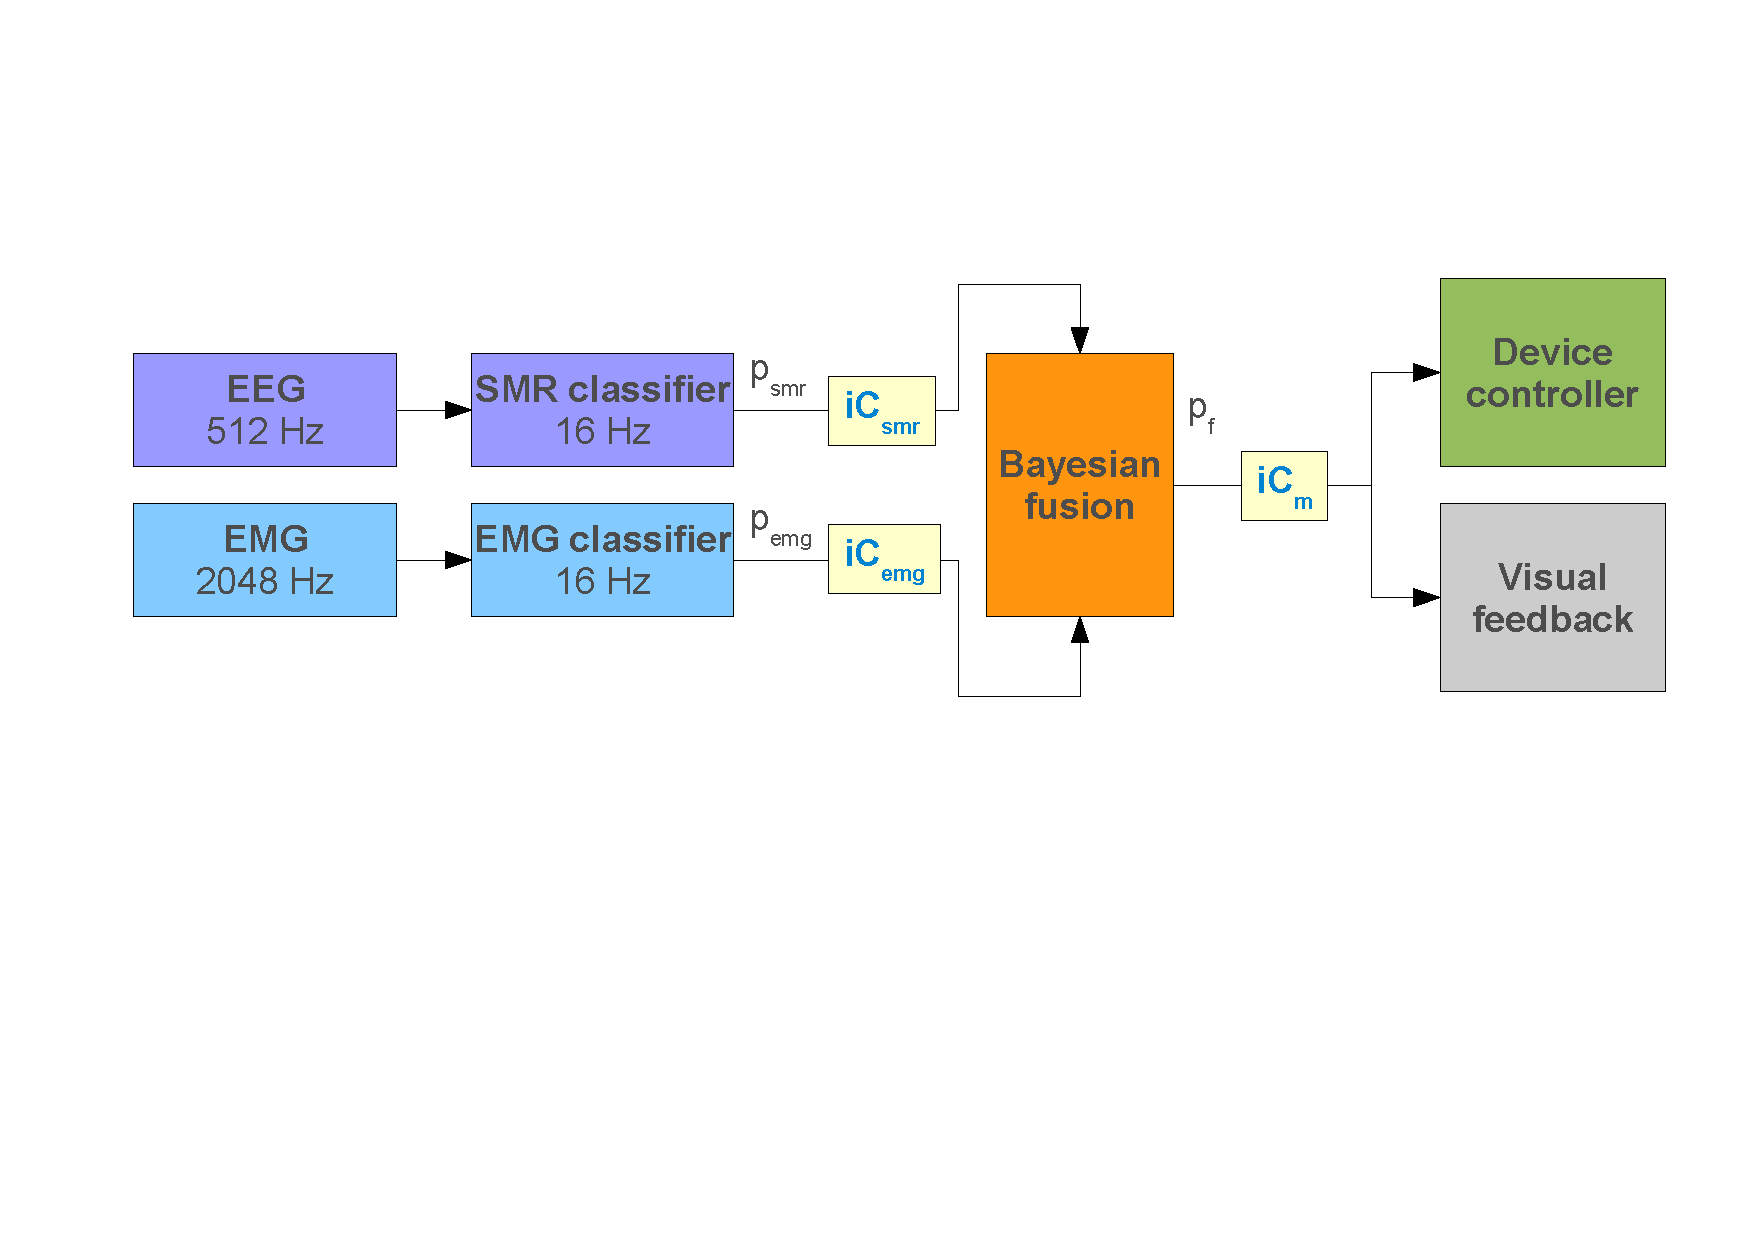
\includegraphics[width=\textwidth]{figures/example1.pdf}
	\caption{The SMR and EMG classifier output $p_{smr}$ and $p_{emg}$
	probabilities, that are transmitted to the fusion block in two iC messages: 
	\temp{$iC_{smr}$} and \temp{$iC_{emg}$}. The fusion emits a probability that
	$p_{f}$, transmitted via \temp{$iC_{f}$}.}
	\label{fig:hbci:example1}
  \end{center}
\end{figure}
Spectral components are then extracted from EEG at 16Hz and classified, 
while EMG activity is classified directly in the time domain and a probability
output is provided at 16Hz.

EEG and EMG activity are classified by two different classifiers, as shown in
Figure~\ref{fig:hbci:example1}.
The two probability outputs, $p_{smr}$ and $p_{emg}$, are sent
in two different iC messages (\temp{$iC_{smr}$} and
\temp{$iC_{emg}$}) to the fusion module. 
The fusion module outputs a single iC message (\temp{$iC_{f}$})
containing the fused probability $p_{f}=f(p_{smr}, p_{emg}$). 

Two points need to be highlighted. First, the classifier output is generally
much slower than the rate biological signals are acquired. Secondly, the output
of a classifier can reach a larger set of modules, for which disparity needs to
be taken in consideration. 
The latter claims motivated the use of TCP/IP communication and XML format for
transmitting and encoding the messages (Section~\ref{sec:implementation}).

\subsection{EEG and ErrP fusion}
\label{sec:hbci:example2}
In the previous example we used the case of EEG and EMG fusion to showcase a
typical example of iC use within the hBCI design. 
Before we were fusing two probabilities in one. From an iC message perspective,
the fusion module receives two distinct messages, extracts the probabilities,
fuse them together and outputs a message with the result of the fusion.

Another possibility might require the fusion to receive multiple iC messages and
combine them together, as in the case of the EEG/ErrPs BCI shown in this
example.
\label{sec:hbci:example2}
\begin{figure}[!htb]
  \begin{center}
	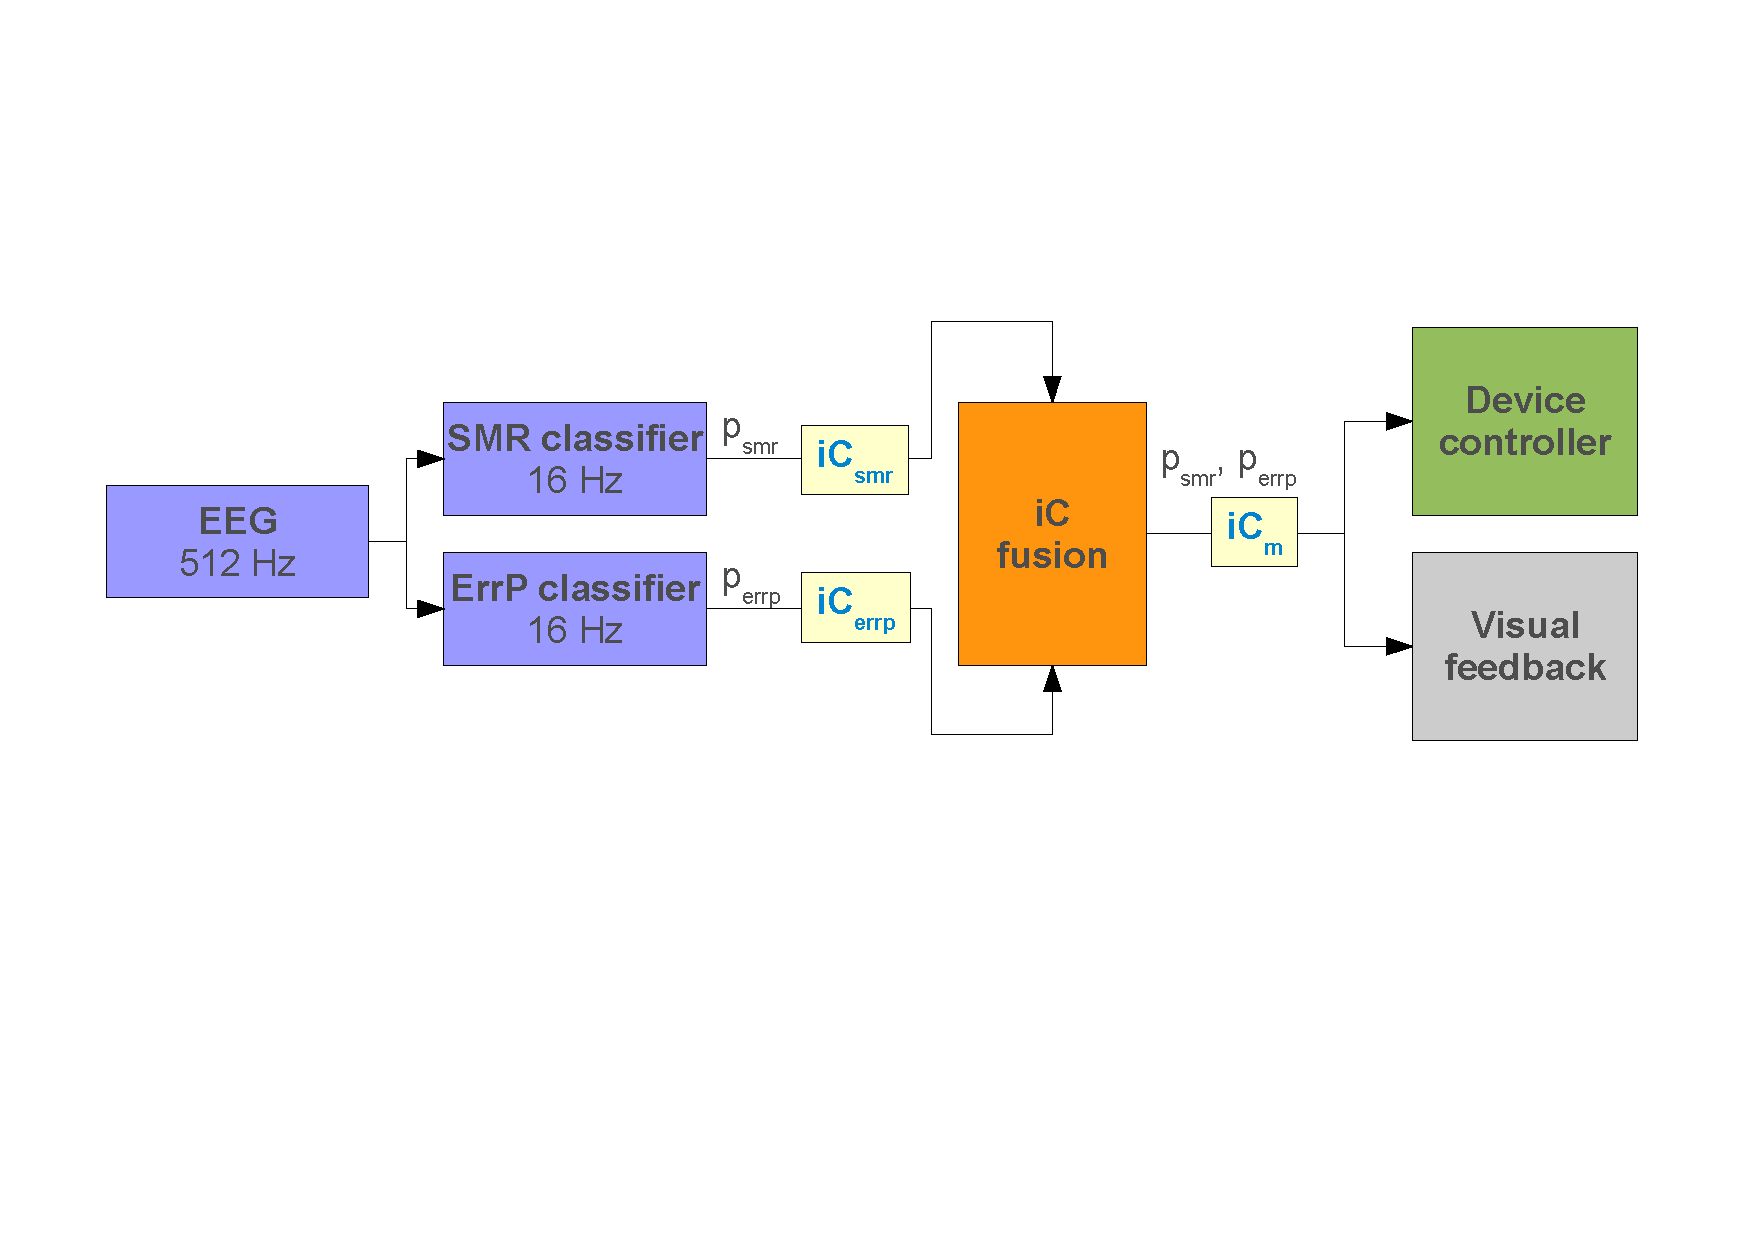
\includegraphics[width=\textwidth]{figures/example2.pdf}
	\caption{The SMR and ErrP classifier output $p_{smr}$ and $p_{errp}$
	probabilities, that are transmitted to the fusion block in two iC messages: 
	\temp{$iC_{smr}$} and \temp{$iC_{emg}$}. The fusion emits a probability that
	$p_{m}$, transmitted via \temp{$iC_{m}$}.}
	\label{fig:hbci:example2}
  \end{center}
\end{figure}

Similarly as before, the fusion receives two probabilities $p_{smr}$ and
$p_{errp}$. The two probabilities are received as two iC messages, 
\temp{$iC_{smr}$} and \temp{$iC_{errp}$} respectively.
This time the fusion module extracts the content of the two input messages and
merges is in a single message, \temp{$iC_{m}$}, containing both received
probabilities ($p_{smr}$ and $p_{errp}$).
The internal structure of \temp{$iC_{m}$} is displayed in
Figure~\ref{fig:hbci:icmessage}.

\section{Structure of an iC message}
\label{sec:icstructure}
It should now be clear to the reader that iC messages are used to have
classifiers communicate with higher level modules. It should also be clear that
iC messages constitute the atomic communication unit of TOBI iC.
Finally, in the two examples we showed how different fusion modules can
manipulate the content of the iC messages in very different ways.

What has not been described yet is the internal structure of an iC message, but
specially the fact that iC can be used directly within your libraries and
programs to describe classifiers, class labels and class values.
In fact, iC is not only a way to encode/decode messages to be streamed in the
hBCI pipeline. Its internal auto-configurable structures make iC the perfect
solution to handle whatever is related to statistics and classification within
any BCI design.
Furthermore, thanks to the TOBI standards, it makes it possible to design
plug-and-play hBCI modules (\note{This is dedicated to WP8 people, but we need
to define the standard somehow}).

Figure~\ref{fig:hbci:icmessage} depicts the internal structure of the iC message
\temp{$iC_{m}$} from the example of Section~\ref{fig:hbci:example2}. 
The diagram provides an ideal schematic for the topics introduced in this
Session. For this reason, we encourage the reader to refer to it throughout the
development of the following paragraphs.

\subsection{iC messages}
\label{sec:icmessage}
An iC message has to be considered as a set of iC classifiers and two
attributes: a frame number and a iC version tag.

When the acquisition feeds in the hBCI pipe a data frame (i.e. EEG, EMG,
etc.), it sets its frame number. Frame numbers are used withing the hBCI design
to make sure data in different pipelines are aligned with each other. 
Not only: frame numbers become really handy to debug the whole loop.
The two last claims become stringent requirements for distributed designs, in
which different modules run on different processes or even machines.

Under this perspective, when a classifier receives some RAW data and outputs
a probability, it must also set the frame number in the iC message so to convey
the acquisition timing information to the higher level modules.

The version tag contains the specific version of TOBI iC. In this way, different
modules that communicate by means of iC, can know if they have all the
capabilities required to decode a received iC message.

As stated few lines ago, apart from the frame number and the version tag, an iC
message has one or more classifiers, described in the next Section.

\subsection{iC classifiers}
\label{sec:icclassifier}
An iC classifier is, by definition, a set of iC classes. So, if you want, the iC
message is like an onion, where each layer stores some kind of information about
a classifier output. More in depth the layer is, more low-level the information
stored wherein will be.

Each iC message stores multiple classifiers using an hash table. An hash table
is a data structure in which a key (i.e. ``red'', ``green'', ``blue'') is
associated to a value (i.e. ``FF0000'', ``00FF00'', ``0000FF'').
In iC, the key of the hash table is the classifier name, and the value is an iC
classifier.

\begin{figure}[!htb]
  \begin{center}
	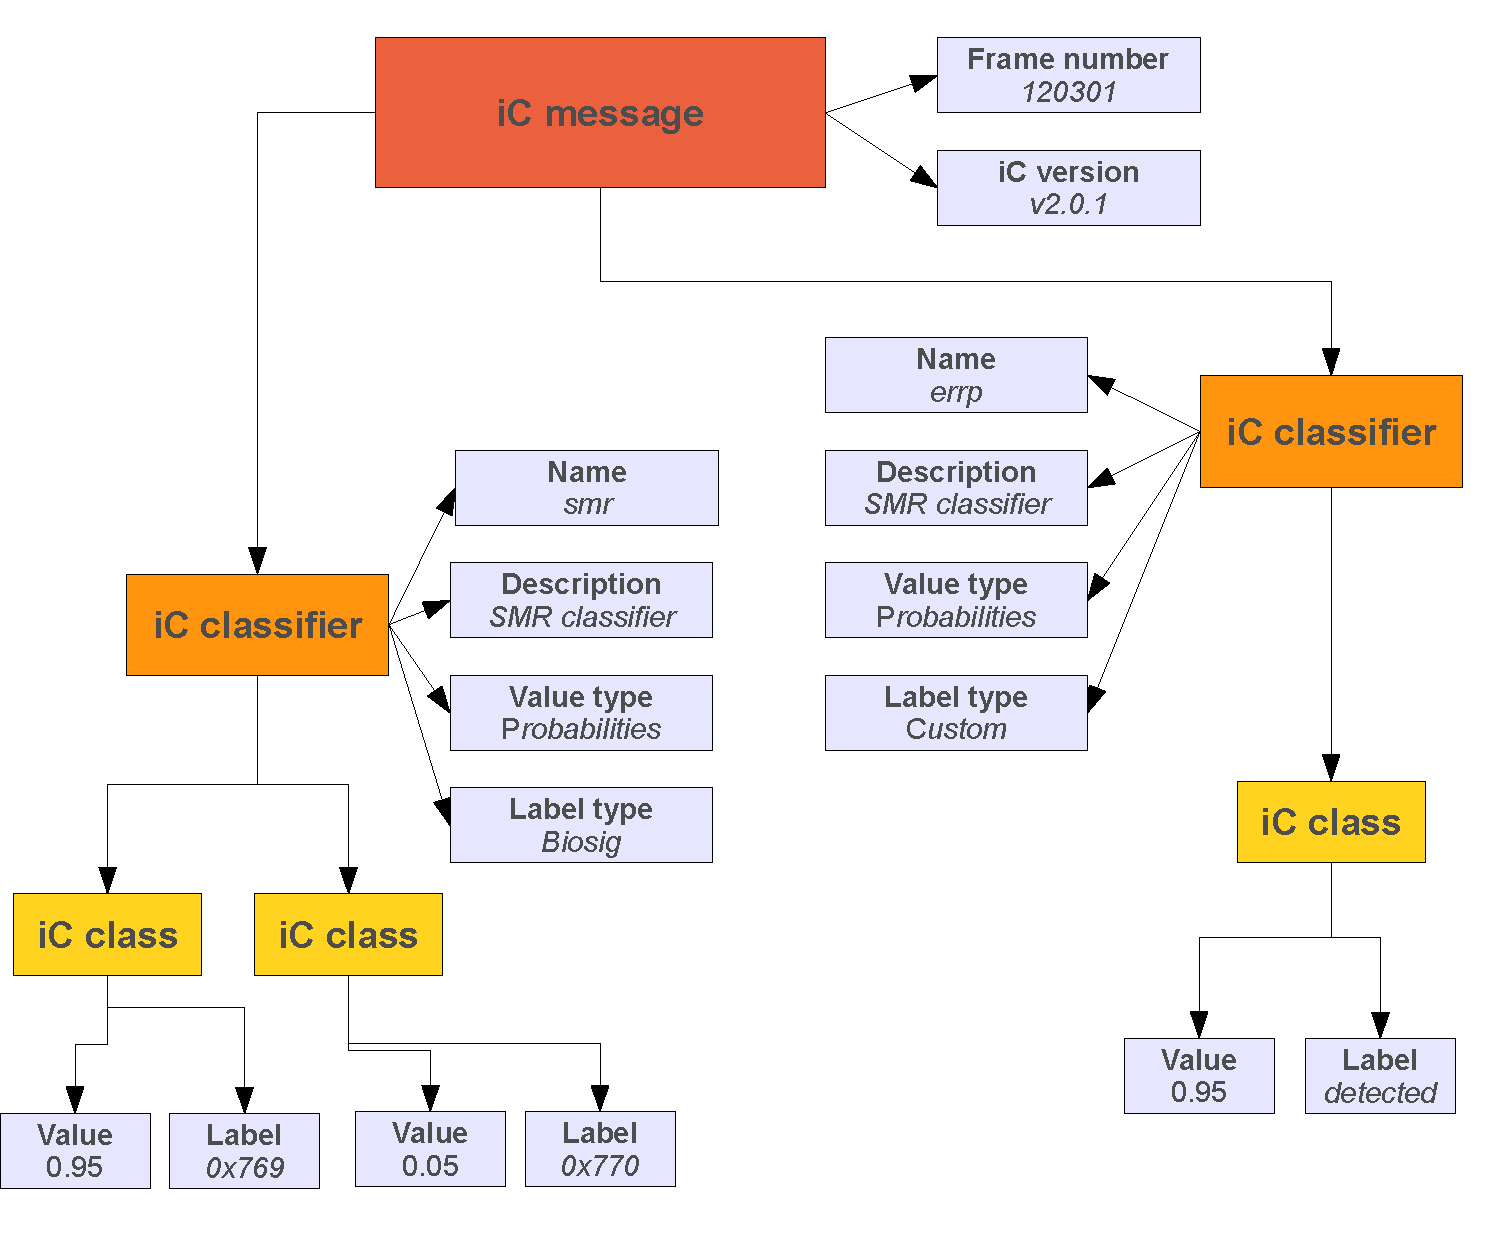
\includegraphics[width=\textwidth]{figures/icmessage.pdf}
	\caption{Internal structure of the iC message \temp{$iC_{m}$} from 
	  Section~\ref{fig:hbci:example2}. The light blue boxes contain the
	  attributes for iC message, iC classifiers and iC classes.}
	\label{fig:hbci:icmessage}
  \end{center}
\end{figure}
\noindent An iC classifier has four distinct attributes:
\begin{enumerate}
  \item {\bf Name}: the name of the classifier (i.e. ``smr'', ``emg'' or
  ``errp''). This attribute is mandatory and acts as a primary key for the hash
  table. Within an iC message, the name of an iC classifier must be unique.
  \item {\bf Description}: the description of the classifier (i.e. ``SMR
  classifier'', ``EMG classifier'' or ``ErrP classifier''). This attribute is
  not mandatory.
  \item {\bf Value type}: the value type attribute describes what kind of output
  is emitted by the classifier. Possible value types are probabilities or 
  regression coefficients.
  \item {\bf Label type}: the label type attribute encodes the type of the class
  labels. For example, an ``smr'' classifier might classify right versus left
  hand or tongue versus both feet motor imagery. This four kinds of motor
  imagery are labeled differently. The label type defines which kind of label it
  will be used for the different kinds of classes. Possible values are custom
  labels (i.e. ``right\_hand\_mi'', ``left\_hand\_mi'') or Biosig labels (i.e.
  ``0x769'', ``0x770''). 
\end{enumerate}


\subsection{iC classes}
\label{sec:icclass}
An iC class is the basic unit of an iC classifier. It stores a class value and a
class label. For example, the ``smr'' classifier encodes values as probabilities
and uses Biosig labels for two classes: right hand  and left hand motor imagery.
The class values could be, for example, 0.05 and 0.95, while the class labels
would be ``0x769'' and ``0x770''.

\section{Implementation}
\label{sec:implementation}
TOBI iC is implemented in C++ and uses GNU Autoconf and Automake to configure
and build the library. The library is platform independent and can be easily
compiled under windows using MinGW + MSys. The University of Glasgow maintains
the Python bindings, while QualiLife maintains the .Net version.
The only external dependency of libtobiic is RapidXML.

A MEX interface for Mathworks Matlab has been written using MWrap. To build the
MEX interface under Microsoft Windows, it is necessary to use MinGW + MSys
together with GNUMex and Mwrap. A precompiled version for Microsoft Windows
32bit is available on the TOBI SVN.

\subsection{Communication}
\label{sec:transport}
As today iC is not shipped with a transport layer (i.e. TCP/IP, UDP) because
different partners within the TOBI consortium use already different networking
stacks. 
If you are not expert in coding and you want to evaluate iC, we strongly
recommend to start with the MEX interface and eventually using jtcp or judp for
sending data on the network.

\subsection{Serialization}
\label{sec:serialization}
Up to now we always said that iC messages are exchanged between different
modules. Still, we never addressed specifically how this messages are encoded
and decoded for the transmission.
Similarly to what has been said in Section~\ref{sec:transport} for the
communication, different groups might require different solutions for
encoding/decoding iC messages.
For this reason the library provides a template class named \emph{ICSerializer}
on top of which is possible to implement any serialization method.

As today the consortium agreed on keeping the complexity of high-level
communication as low as possible, thus choosing XML (using RapidXML as a
back-end) for the serialization and de-serialization of the iC messages.
Readers interested in this topic will find all the necessary informations in
Section~\ref{sec:examples}.

Some examples of serialized iC messages are available in
Section~\label{sec:code:example1}.

\subsection{libtobiic}
\label{sec:libtobiic}
The C++ library is distributed with a Doxygen API documentation and several
examples. It can be downloaded from here: \small{\texttt{http://}}.

\subsection{mextobiic}
\label{sec:mextobiic}
The MEX interface is distributed with the standard Mathworks Matlab
documentation and several examples. It can be downloaded from here:
\small{\texttt{http://}}.

\subsection{Limitations of mextobiic}
\label{sec:limitations}
Although the Matlab interface provides all the means to manipulate the hierarchy
of the iC structures, it does not allow the user to perform complex automated
operations to combine and merge messages together. 
This is evident in Section~\ref{sec:examples}, where fusion is handled manually.
As today it is still unclear to what extent this functionality will be
implemented in the core library and exposed in the MEX interface. 
Still, the libtobiic API is ready for all possible message manipulations, and in
C++ it is trivial to perform such kind of operations. Under a usability
perspective, the maintainers will add soon some extra functionality to support
the automated merging and splitting of iC messages.

\section{Examples}
\label{sec:examples}
The examples in the following Sections implement and comment, line by line, what
has been described in Section~\ref{sec:hbci:example1}
and~\ref{sec:hbci:example2}. The examples here provided are coded in Matlab.

\subsection{EEG and EMG fusion}
\label{sec:code:example1}
The code for the first example is included directly in this document. Still, the
reader should be aware that the example is distributed with mextobiic. The
comments are provided as in the example.

To help the reader, these are the main functional blocks within the provided
example:
\begin{itemize}
  \item Lines 19-35: configuration of the SMR iC message \temp{$iC_{smr}$},
  classifier and classes.
  \item Lines 38-54: configuration of the EMG iC message \temp{$iC_{emg}$},
  classifier and classes.  
  \item Lines 57-85: configuration of the Fusion iC message \temp{$iC_{f}$},
  classifier and classes both for the inputs and for the output.
  \item Lines 91-172: simulated hBCI loop (from the classifier output to the
  fusion output only).
  \begin{itemize}
	\item Lines 92-98: setting of frame number
	\item Lines 100-110: setting of the class values
	\item Lines 112-139: serialization and de-serialization of the iC messages
	\item Lines 141-153: fusion of the probabilities emitted by the classifiers
  \end{itemize}
  \item Lines 174-185: de-allocation of the iC objects
\end{itemize}
The XML messages, resulting from the serialization of the different iC messages,
can be found in Section~\ref{sec:code:example1:emg}, \ref{sec:code:example1:smr}
and~\ref{sec:code:example1:fusion}.
\lstinputlisting{mat/example1.m}

\subsubsection{XML message for the SMR classifier}
The serialized version of an iC message for the SMR classifier is here provided.
\label{sec:code:example1:smr}
\lstinputlisting{xml/example1_smr.xml}

\subsubsection{XML message for the EMG classifier}
\label{sec:code:example1:emg}
The serialized version of an iC message for the EMG classifier is here provided.
\lstinputlisting{xml/example1_emg.xml}

\subsubsection{XML message for the Fusion module}
\label{sec:code:example1:fusion}
The serialized version of an iC message for the Fusion module is here provided.
\lstinputlisting{xml/example1_fusion.xml}

\subsection{EEG and ErrP fusion}
\label{sec:code:example2}
This example follows what already seen in Section~\ref{sec:code:example1}. The
only difference is the merging of the classifier outputs and the configuration
of the iC message emitted by the fusion (Lines 141-148 and 55-80 respectively).
Furthermore, the reader might be interested in comparing the XML output in
Section~\ref{sec:code:example2:fusion} with the one in
Section~\ref{sec:codmat/e:example1:fusion}.
\lstinputlisting{mat/example2.m}

\subsubsection{XML message for the Fusion module}
\label{sec:code:example2:fusion}
The serialized version of an iC message for the Fusion module is here provided.
\lstinputlisting{xml/example2_fusion.xml}
\end{document}
